\documentclass{article}

\usepackage{pandekten}

\title{\texorpdfstring{$\Phi^4$ Theory}{Phi4 Theory}}
\author{Ch\=an Taku}

\begin{document}

\maketitle

\section{Gallery}

\begin{proposition}{1-Loop Coorrection of Vertex}{1_loop_correction_of_vertex}
    \[ 
        \arraycolsep=0pt
        \begin{array}{lll}
            \qty(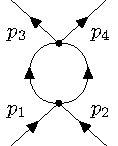
\includegraphics[valign=c]{img/s-22/s-22.pdf})_{\operatorname{D}(d)} & \qty(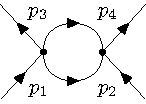
\includegraphics[valign=c]{img/t-22/t-22.pdf})_{\operatorname{D}(d)} & \qty(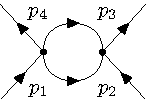
\includegraphics[valign=c]{img/u-22/u-22.pdf})_{\operatorname{D}(d)} \\
            = (-i\lambda)^2 iV(s); & = (-i\lambda)^2 iV(t); & = (-i\lambda)^2 iV(u);
        \end{array}
    \]
    where
    \[ V(p^2) = -\frac{1}{2} \int_0^1 \dd{x} \frac{\Gamma(2-d/2)}{(4\pi)^{d/2}} \frac{1}{\qty[m^2 - x(1-x)p^2]^{2-d/2}}, \]
    and $s,t,u$ are the Mandelstam variables of the process $\ket{p_1,p_2}\rightarrow \ket{p_3,p_4}$, respectively.
    Dropping terms of $\bigO(\epsilon)$ we find
    \[ V(p^2) = -\frac{1}{32\pi^2} \int_0^1 \dd{x} \qty(\frac{2}{\epsilon} - \gamma + \log(4\pi) - \log\qty[m^2 - x(1-x)p^2]). \]
\end{proposition}

% \bibliographystyle{plain}
% \bibliography{main}

\end{document}
